\documentclass[exam,addpoints, noanswers]{exam}

\usepackage[exam]{physics9}

\title{Test \#3A}
\date{\today}
\author{\mobeardInstructorShort}
% retest for Ashleigh Schubert

\begin{document}
\maketitle
\vfill
\mobeardExamNameBlock
\vfill
Instructions: 
\begin{enumerate}
\item Do not open exam until instructor announces that you may begin.
\item Please write your name on each page in case the sheets are separated. 
\item Closed notes, closed book.  You may use two \SI{8.5x11}{\inch} note sheets, both sides. 
\item Calculators (TI-84 or equivalent) are permitted.  On standardized tests you will not be permitted to use your cell phone as a calculator, so it is best to get used to your calculator now. 
\item Eight multiple choice are worth five points each, two essay questions (divided into parts) are worth 30 points each.  \textbf{The test format is the same as the previous Q3 test}. 
\item In answering the essay questions, be thorough but concise. Deep understanding of the concepts will be displayed by proper use of vocabulary and discussion of the interconnectedness of concepts. 
\item Show your calculations and (most importantly) your \textbf{thinking}.
\end{enumerate}
\vfill
\begin{center}
\gradetable[h][questions]
\end{center}
\clearpage



\begin{questions}
\question[5] Which of the following about scalars and vectors is true? Please select all that apply. 
\begin{choices}
\choice A scalar has magnitude and direction while a vector has magnitude only. 
\CorrectChoice A scalar has magnitude only while a vector has magnitude and direction. 
\CorrectChoice A scalar times a vector is a vector. 
\choice A scalar times a scalar is a vector, because it has two numbers. 
\CorrectChoice Vectors can be subtracted from vectors. 
\end{choices}



\question[5] Xuan the puppy walks in a circle of radius $r$ and returns to his starting point. Which of the following is true? Please show your work.
\begin{choices}
\choice Xuan's distance is zero and his displacement is $2\pi r$. 
\choice Xuan's distance is zero and his displacement is $\pi r^2$. 
\CorrectChoice Xuan's distance is $2\pi r$ and his displacement is zero. 
\choice Xuan's distance is $\pi r^2$ and his displacement is zero. 
\choice Xuan's distance is $r$ and his displacement is $-r$, since he returned to the same place. 
\end{choices}



\question[5] Which of the following are part of Newton's laws? Please select all that apply.  
\begin{choices}
\choice Around a closed loop, the sum of the drops is equal to zero. 
\CorrectChoice The sum of the forces is equal to the time rate of change of momentum. 
\choice At a node, the sum of the currents flowing into the node is zero. 
\CorrectChoice An object at rest will stay at rest unless acted upon by an outside force. 
\CorrectChoice $F=ma$. 
\end{choices}


\clearpage
\question[5]\label{q4} The plots in \fref{fig:q4} show data from drop tests on another planet. The person who did the plots forgot to label the $y$ axes. Assuming the units used in the plot are standard metric (SI) units, which statements are true? Please select all that apply. 
\begin{choices}
\choice A shows the position and B shows the velocity. 
\CorrectChoice A shows the velocity and B shows the position.
\CorrectChoice The slope of the line in A gives the acceleration of gravity on the planet. 
\CorrectChoice The shape of the velocity is linear. 
\choice The acceleration of gravity is approximately \SI{0.98e1}{\meter\per\second\squared}. 
\end{choices}
\setcounter{figure}{3}
\begin{figure}[h]
\begin{center}
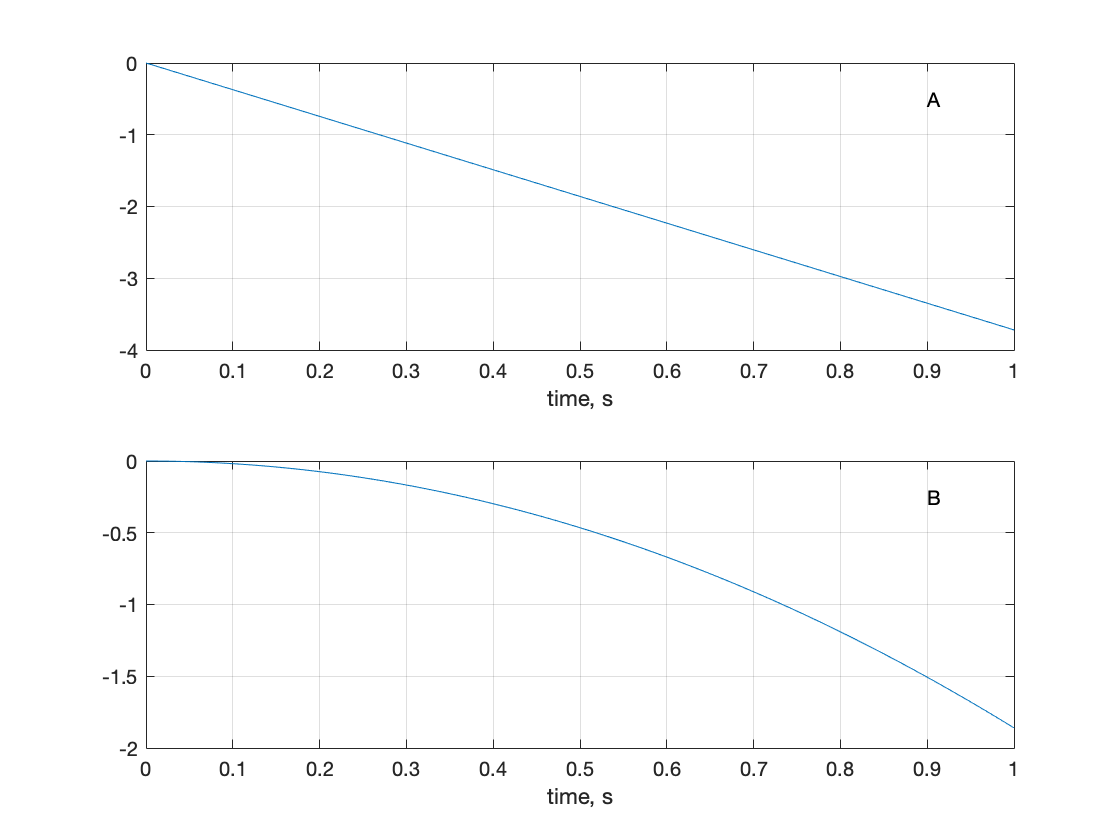
\includegraphics[width=5in]{Q3Aq4.png}
\end{center}
\caption{Question~\ref{q4}}
\label{fig:q4}
\end{figure}


\clearpage
\question[5]\label{q5} ``Give me a lever long enough and a fulcrum on which to place it, and I shall move the world.''  The figure below shows a simple machine called a lever in use. Apply Newton's laws and sketch a free body diagram of the isolated lever (the beam in \fref{fig:q5}). You do \textbf{not} have to solve for the forces. 
\begin{solution}[5in]
\end{solution}
\setcounter{figure}{4}
\begin{figure}[h]
\begin{center}
\includegraphics[width=3in]{parts-of-a-lever.jpg}
\end{center}
\caption{Question~\ref{q5}. The lever is the red beam. }
\label{fig:q5}
\end{figure}

\clearpage
\question[5] You are checking your friend's physics homework. Without checking their calculations, which answers are most definitely WRONG? Please select all that, without a doubt, have something wrong with them
\begin{choices}
\CorrectChoice velocity = \SI{1.2}{\meter\per\second} 
\CorrectChoice acceleration = \SI{9.81}{\meter\per\second\squared} 
\CorrectChoice $x = \SI{5}{\newton}$ 
\CorrectChoice distance = \SI{32767}{\meter\per\second}
\choice force = \SI{1500}{kip}, in compression
\choice mass = \num{7840} slug
\choice speed = \num{42} knots
\CorrectChoice Weight is equal to \SI{9.81}{\foot\per\second\squared} times the mass. 
\CorrectChoice Using a stopwatch, the measured speed of the car as it drove around the track was $v=\SI{3.14159265358979}{\meter\per\second}$. 
\end{choices}




\question[5] Dr Evangelista is driving at \SI{10}{\meter\per\second} when he sees a cat \SI{100}{\meter} in front of him. He immediately hits the brakes and begins decelerating at \SI{10}{\meter\per\second\squared}. In what distance does he come to a stop, and why? 
\begin{choices}
\CorrectChoice \SI{5}{\meter}, using $x = \dfrac{1}{2} a t^2 + v_0 t + x_0$ and $v = a t + v_0$. 
\choice \SI{1}{\second}, using $v = a t + v_0$
\choice \SI{5}{\meter}, using $v=a t + v_0$
\choice \SI{-50}{\meter}, using $x = \dfrac{1}{2} x_0 t^2 + v_0 t + x_0$
\choice It is impossible to determine how long it takes him to stop without knowing $x_0$
\end{choices}



\clearpage
\question[1]\label{q8} For the plot below, determine the velocity.  
\begin{choices}
\choice \SI{6}{\meter\per\second}
\choice \SI{-3}{\meter\per\second}
\choice \SI{1}{\meter\per\second}
\CorrectChoice \SI{3}{\meter\per\second}
\choice The plot gives position, so velocity cannot be determined. 
\end{choices}
\setcounter{figure}{7}
\begin{figure}[h]
\begin{center}
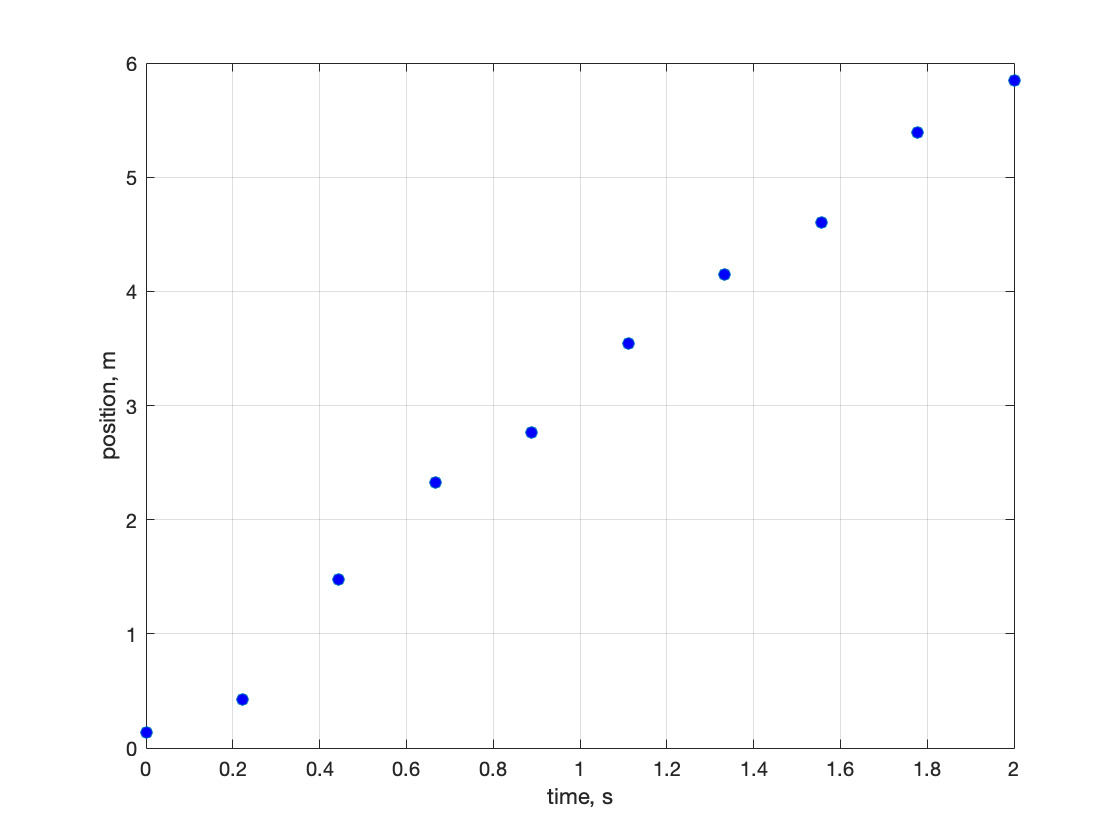
\includegraphics[width=5in]{Q3Aq8.png}
\end{center}
\caption{Question~\ref{q8}}
\label{fig:q8}
\end{figure}




\clearpage
\question\label{q9} The Mars Helicopter Ingenuity (\fref{fig:q9}) is a small (\SI{1.8}{\kilo\gram}) solar-powered helicopter with counter-rotating blades that spin at about \SI{2400}{\rpm}. It is equipped with computers, navigation sensors, and two cameras. The height is \SI{0.49}{\meter} and the span is \SI{1.2}{\meter}. It is deployed from the Mars Rover Curiosity (\SI{899}{\kilo\gram}). 
\begin{figure}[h]
\begin{center}
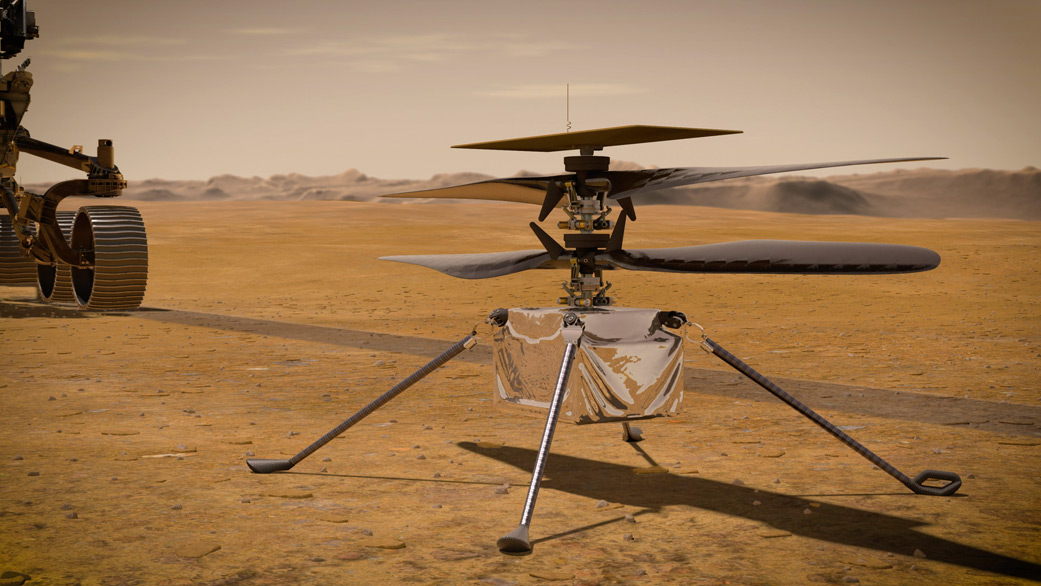
\includegraphics[width=1.5in]{ingenuity.jpg}
\end{center}
\caption{Question~\ref{q9}}
\label{fig:q9}
\end{figure}
\begin{parts}
\part[5] Assume the Ingenuity has taken off, is out of ground effect, and is translating steadily upwards at \SI{0.5}{\meter\per\second}. Draw a free body diagram of the Mars Helicopter Ingenuity.
\begin{solution}[3in]
\end{solution}

\part[5] Write the equations of motion (kinematics) that apply during this type of motion. 
\begin{solution}[2in]
\end{solution}

\clearpage
\part[5] If the acceleration of gravity on Mars is \SI{-3.38}{\meter\per\second\squared}, what is the weight of the Mars Helicopter Ingenuity, and how much upward force must the rotors generate during this flight condition?
\begin{solution}[1.5in]
\end{solution}

\part[5] The onboard computers detect a fault and go into an emergency state where the craft descends under \textbf{autorotation}. During autorotation at the autorotation speed, the rotors ``windmill'' and generate enough lift to counteract the weight. Draw a free body diagram of the Mars Helicopter Ingenuity during this state. 
\begin{solution}[3in]
\end{solution}

\part[5] If the acceleration of gravity on Mars is \SI{-3.38}{\meter\per\second}, what is the overall acceleration of the craft once it reaches the autorotation speed? 
\begin{solution}[1in]
\end{solution}

\part[5] What are the relevant equations of motion (kinematics) for the craft once it reaches the autorotation speed? 
\begin{solution}[1in]
\end{solution}
\end{parts}

\clearpage
\question For the second short answer question, you get a job at NASA working on a small, zero G robot propelled with compressed air, able to move around inside the International Space Station. You are planning a set of commands to transmit to the robot for an upcoming flight test on a ``Vomit Comet'' C-9B microgravity simulator plane. 

\begin{parts}
\part[10] The first test maneuver is to fly up \SI{1}{\meter} in \SI{1}{\second}, hover for 
\SI{1}{\second}, then return to the launch point in \SI{1}{\second}. In the space here, sketch the vertical position and velocity of the robot. (You will need this to construct velocity commands to send to the robot, and to set failsafe limits on position in its autonomous flight controller.) 
\begin{solution}[6in]
\end{solution}

\clearpage
\part[10] During the actual test, a failure occurs in the propulsion system, resulting in the throttle valve being stuck open during the first part of the maneuver (heading upwards). With the failed valve, the force on the robot is \SI{10}{\newton} and its mass is \SI{1}{\kilo\gram}. Please plot the robot's position versus time. The far wall of the test chamber is \SI{10}{\meter} away; show when it hits the wall on your graph. Assume the robot is streamlined so that air resistance is small and neglect any change in mass from the expulsion of propellant.  
\begin{solution}[6in]
\end{solution}

\clearpage
\part[10] To think about design changes in case of another similar failure, we need to know how long the robot has to respond, and how bad it is when it hits. Please compute the time to hitting the wall, and the speed when it hits. 
\begin{solution}[6in]
\end{solution}
\end{parts}
\end{questions}
\end{document}